\chapter{Architecture}
\label{chap:architecture}


\begin{chapterintro}
This chapter describes in depth how the system is structured in different modules and how the users interact with them and also how the modules interact with other modules by themselves.
\end{chapterintro}

\cleardoublepage
\section{Architecture Overview}
In this section we will describe the \textbf{videogame architecture}, starting with its two main modules, the \textbf{physical instruments miniatures} and the \textbf{software application}. In Figure \ref{fig:ArchitectureGeneral} we show the global game architecture identifying both main modules and their relation.

\begin{figure}[ht!]
	\centering
	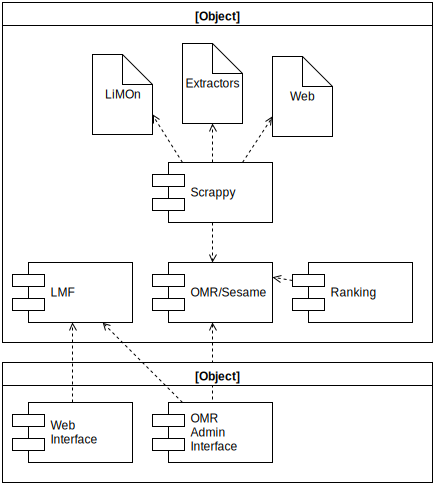
\includegraphics[width=400pt]{graphics/ArchitectureGeneral.pdf}
	\caption{General Architecture}
	\label{fig:ArchitectureGeneral}
\end{figure}

\FloatBarrier

The modules are detailed below:

\subsection{Physical instruments miniatures}
There are five physical miniatures which represents each one of the musical instrument families used at the game: percussion, keyboards, strings, woodwind and brass. The gamer will use these pieces to interact with the app in order to change or activate the family represented by the piece. Also, pieces will be used to access to different game modes.

The interaction between the pieces and the app is haptic, that is, the gamer will pick a miniature and they will place it in the “instrument detection zone” represented by a shiny circle in the app screen. The app “detection algorithm” will determine which piece has been placed and will make an event depending on the game mode and the app state. These events are, for example, changing instrument, activate instrument, etc.

Each piece base has three little pads which conform a triangle used to determine the instrument unequivocally.

Instrument miniatures design will be explain in more detail in section \ref{sec:instrumentminuatures}

\subsection{Application}
The application have been developed using Unity, so we can identify the Unity components included on our app. These components are Unity Scenes, Unity Textures, Unity Assets, Unity Scripts and Unity Sounds. Integrating all of these components into our Unity projects we are able to build the game logic and its graphic interface.

Unity is notable for its ability to target games to multiple platforms. Within a project, we have control over delivery to different mobile devices, web browsers, desktops, and consoles. In our case, we need to develop both Android and iOs applications and Unity allow us to share the same code for them. Also, using Unity Android and iOs Plugins we are able to access to native Android and iOs SDKs, in case we need to access to some Android or iOs native components.

The application archiecture will be explain in more detail in section \ref{sec:application}

\FloatBarrier

\section{Physical instruments miniatures}
\label{sec:instrumentminuatures}
\#Escribir sobre el diseño de los pads en las bases de las piezas para su detección (también sobre el algoritmo de detección)

\FloatBarrier

\section{Application}
\label{sec:application}
The application is the biggest module of the game. It includes the whole software development as it is shown in Figure \ref{fig:applicationarquitecture}.

\begin{figure}[h]
	\centering
	\includegraphics[width=400pt]{graphics/Application_arquitecture.pdf}
	\caption{Application arquitecture diagram}
	\label{fig:applicationarquitecture}
\end{figure}

If we look at the application architecture diagram we can see the Application module where Unity game engine will run. Unity has three main components, Unity Assets, Unity Scripts and Unity Scenes, which are described below:

\subsection{Assets}
An asset is representation of any item that can be used in your game or project. An asset may come from a file created outside of Unity, such as a 3D model, an audio file, an image, or any of the other types of file that Unity supports. There are also some asset types that can be created within Unity, such as an Animator Controller, an Audio Mixer or a Texture Managers. In other words, assets are any resource your game uses.

Thankfully, Unity’s asset importing is robust and intelligent, it will accept all popular 3D file formats and also supports all common image file formats, including PNG, JPEG, TIFF and even layered PSD files directly from Photoshop. When it comes to audio, Unity supports WAV and AIF, ideal for sound effects, and MP3 and OGG for music.

In Figure \ref{fig:applicationarquitecture} we can see that sounds and textures are included as assets to use them, but they are not the only assets we will use. We said that there are some assets types that have been created within Unity to make development easier. In our case we will use an Animation Controller called HOTween, a 2D Texture Manager called 2dToolkit and both Android and iOs plugins. All these assets are included in our Unity project downloading them from Unity Asset Store.

The Unity Asset Store is home to a growing library of free and commercial assets created both by Unity Technologies and also members of the community. A wide variety of assets is available, covering everything from textures, models and animations to whole project examples, tutorials and Editor extensions. These assets are accessed from a simple interface built into the Unity Editor and are downloaded and imported directly into your project.

Assets will be used from the Scenes and/or the Scripts, which are detailed in section \ref{subsec:unityscripts}.

\subsection{Scenes}
Scenes contain the objects of your game. They can be used to create a main menu, individual levels, and anything else. Each unique Scene file as a unique level, where you will place your environments, obstacles, and decorations, essentially designing and building your game in pieces.

We can easily make an analogy between Scenes and screens in our app. Each screen is built from a Scene where all the Assets logic are managed by the Scripts.

Creating Scenes with unity are possible thanks to their intuitive interface, where project assets can be drag to the interface Scene and Scripts can be attached to the assets to control them.

\subsection{Scripts}
\label{subsec:unityscripts}
Scripts, known in Unity as behaviours, let you take assets in your scene and make them interactive. Multiple scripts can be attached to a single object, allowing for easy code reuse. Unity supports three different programming languages; UnityScript, C\#, and Boo. In our project we will use C\#.

As we can see in Figure 3.2, Scripts will manage Unity Assets and will use external Assets from the Unity Asset Store as libraries to make the development easier. In our case, HOTween asset allow us to automate the animation of any numeric (and some non-numeric) property or field (numbers, vectors, transforms, and so on) in many different ways. 2dToolkit provide an efficient 2D sprite, collider set-up and text system which integrates seamlessly into the Unity environment. Android and iOs plugins allow us to access to native Android and iOs libraries.

As we said, scripts will be attached to the scene assets we need to provide them the functionality we need to.


\section{Application use workflow}
The application has three game modes, for each one we will see the application use workflow to get a more precise idea of how the Gamer will interact with the application.

The three game modes were designed as a result of the Game modes use case defined in section \ref{subsec:gamemodes}:

\begin{itemize}
\item \textit{Playing instrument game mode} detailed in sub-section \ref{subsec:playinstrument_arch}.
\item \textit{Conducting orchestra game mode} detailed in sub-section \ref{subsec:conducteorchestra_arch}.
\item \textit{Discovering instrument game mode}  detailed in sub-section \ref{subsec:discoverinstrument_arch}.
\end{itemize}

\newpage
\subsection{Playing instrument game mode}
\label{subsec:playinstrument_arch}

Playing instrument game mode workflow is represented in Figure \ref{fig:playingworkflow}

\begin{figure}[ht!]
	\centering
	\includegraphics[width=400pt]{graphics/PlayingGameMode.pdf}
	\caption{Playing instrument game mode}
	\label{fig:playingworkflow}
\end{figure}

\FloatBarrier

\newpage
\subsection{Conducting orchestra game mode}
\label{subsec:conducteorchestra_arch}

Conducting orchestra game mode workflow is represented in Figure \ref{fig:conductingworkflow}

\begin{figure}[ht!]
	\centering
	\includegraphics[width=400pt]{graphics/ConductingGameMode.pdf}
	\caption{Conducting orchestra game mode}
	\label{fig:conductingworkflow}
\end{figure}

\newpage
\subsection{Discovering instrument game mode}
\label{subsec:discoverinstrument_arch}

Discovering instrument game mode workflow is represented in Figure \ref{fig:discoveringworkflow}

\begin{figure}[ht!]
	\centering
	\includegraphics[width=400pt]{graphics/DiscoveringGameMode.pdf}
	\caption{Discovering instrument game mode}
	\label{fig:discoveringworkflow}
\end{figure}

\FloatBarrier


\section{Conclusions}

